paragraph{Examples with Predication: }

Now some examples involving control dependencies are
examined.  Consider the following code sequence.

\begin{verbatim}

00	r2 <- r1 op r0
10	b_op r2, 030
20	r3 <- r1 op r0
30	r4 <- r1 op r0

\end{verbatim}

This example illustrates a simple minimal control dependency
situation.
Instruction 30 does not depend, either through a data flow dependency
of a control flow dependency on any of the instructions that
are shown to be before it.  The branch instruction 10 is data
dependent on instruction 00 (through register
{\tt r2}.
And instruction 20 is control
dependent on instruction 10 (the branch).

We start by assuming that all instructions execute in a single clock
cycle and that they all execute immediately upon being loaded.
It is assumed that the initial execution of the branch in
instruction 10 (at time 0) did not change its predicate output.
However, since instruction 00 executed in clock cycle 0, we will
assume that its output value changed from what was originally loaded
at instruction load time.  Instruction 00 will broadcast forward
its new updated output (
register
{\tt r2}).
Since instruction 10 (the branch) is data dependent on
register
{\tt r2}
from instruction 00, it will snoop for that update
and snarf the new value.  This will enable it to re-execute.
We assume that it executes at the earliest possible time.
This would be clock cycle 1.  On this execution, its output predicate,
essentially its branch prediction, does change.  The branch may either
have been resolved at this point or simply may have made a new prediction
based on a possibly still speculative value of register
{\tt r2}.
Either case is handled the same.
A change in the branch condition will change its
predication output and this will be
broadcast out.
Instruction 20, being control dependent on the branch, will be snooping
for this predicate change and seeing that it has changed
will either become enabled for re-execution or re-broadcast
its relay output value.  Which is done depends on the original
the branch prediction and the new action will be the opposite
of the original action taken on the original prediction.
It is assumed that instruction 20 re-executes and it does so
in clock cycle 2.

In spite of the branch being predicted one way and then changed
to the other (whether re-predicted or resolved), it should be
noted that instruction 30 was not required to be re-executed as
a result.  This illustrates a basic minimal control dependency
which serves to facilitate higher instruction level parallelism (ILP)
by taking advantage of independent instruction located beyond the
joins of branches domains.
The execution sequence of this example is shown
in Figure
Figure~\ref{pex1}.

\begin{figure}
\centering
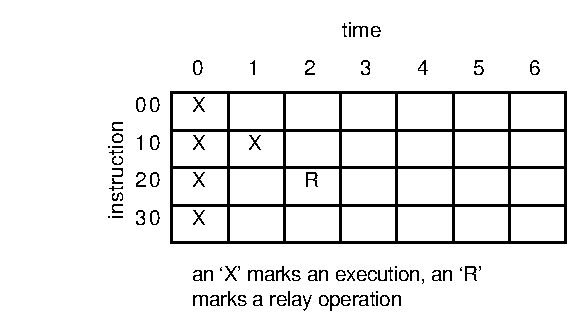
\epsfig{file=pex1.eps,width=2.50in}
\caption{{\em Timing of the code example, predication scenario 1.}
This example illustrates a basic minimal control
dependency, a significant contribution to
achieving higher ILP by taking advantage of independent
instructions beyond the joins of branches.
Execution of an instruction at a given time is
again indicated by an `X'.}
\label{pex1}
\end{figure}

